\documentclass[a4paper]{article}
\usepackage[utf8]{inputenc}
\usepackage[french]{babel}
\usepackage[T1]{fontenc}
\usepackage{lmodern}
\usepackage[left=2cm,right=2cm,top=2cm,bottom=2cm]{geometry}
\usepackage{graphicx}
\usepackage{subfigure}
\usepackage{enumitem}
\usepackage{stmaryrd}
\usepackage{amsmath}
\usepackage{amssymb}
\usepackage{amsthm}
\usepackage{multicol}
\usepackage[hidelinks]{hyperref}
\usepackage{color}
\usepackage{pdfpages}
\usepackage{ebproof}
\usepackage{minted}
\usepackage{manfnt}
\usepackage[bottom]{footmisc}

\usepackage{libertine}
\renewcommand\ttdefault{cmtt}

\usemintedstyle{tango}

\DeclareUnicodeCharacter{393}{$\Gamma$}
\DeclareUnicodeCharacter{22A2}{$\vdash$}
\DeclareUnicodeCharacter{2203}{$\exists$}
\DeclareUnicodeCharacter{2200}{$\forall$}
\DeclareUnicodeCharacter{2208}{$\in$}
\DeclareUnicodeCharacter{3C4}{$\tau$}
\DeclareUnicodeCharacter{3C3}{$\sigma$}

\makeatletter
\AtBeginEnvironment{minted}{\dontdofcolorbox}
\def\dontdofcolorbox{\renewcommand\fcolorbox[4][]{##4}}
\makeatother

\newcommand{\N}{\ensuremath{\mathbb{N}}}
\newcommand{\Z}{\ensuremath{\mathbb{Z}}}
\newcommand{\Q}{\ensuremath{\mathbb{Q}}}
\newcommand{\znz}{\ensuremath{\mathbb{Z} / n \mathbb{Z}}}
\newcommand{\G}{\Gamma}
\DeclareMathOperator{\fv}{\mathrm{fv}}
\DeclareMathOperator{\bv}{\mathrm{bv}}
\DeclareMathOperator{\Succ}{\mathrm{Succ}}
\renewcommand{\epsilon}{\varepsilon}
\renewcommand{\leq}{\leqslant}
\renewcommand{\geq}{\geqslant}
\newcommand{\defi}{\overset{\text{def}}{=}}
\newcommand{\PA}{\mathsf{PA}}
\newcommand{\HA}{\mathsf{HA}}
\newcommand{\ZF}{\mathsf{ZF}}
\newcommand{\NJ}{\mathsf{NJ}}
\newcommand{\NK}{\mathsf{NK}}

\newcommand{\fonc}[5]{#1 : 
\left|
\begin{array}{ccc}
#2 & \longrightarrow & #3 \\
#4 & \longmapsto & #5
\end{array}
\right.
}

\usepackage{titlesec}
\titleformat*{\section}{\center\bf\Large\sffamily}
\titleformat*{\subsection}{\center\bf\large\sffamily}
\titleformat*{\subsubsection}{\center\bf\sffamily}

\setcounter{tocdepth}{2}

\title{Extensions d'un cours de logique du premier ordre certifié en Coq}
\author{Samuel Ben Hamou}
\date{\today}

\begin{document}
%\begin{center}
	%\vspace*{2em}
	
\includegraphics[scale=0.45]{logo_ens.png} %\hspace*{1cm}
	\hfill 
\includegraphics[scale=0.1]{logo-irif.png} \\
\begin{center}
	\vspace*{0.5em}
    %\vspace*{6em}
    {\LARGE Rapport de stage} \\ \vspace{1em}
    {\huge Extensions d'un cours de logique du premier ordre certifié en Coq} \\ \vspace{1.5em}
    
    {\Large Stage effectué du 1 juin au 17 juillet 2020} \\ \vspace{2em}
    
    {\Large Samuel Ben Hamou} \\ \smallskip
    {\large \'Ecole Normale Supérieure Paris-Saclay} \\ 
    {\large 1ère année, Département Informatique} \\ \vspace{1.5em}
    
    {\Large Sous la supervision de Pierre Letouzey} \\ \smallskip
    {\large IRIF, INRIA et CNRS} \vspace{1em}
\end{center}


\begin{abstract}
Ce stage de recherche de fin de licence avait pour but de proposer des extensions à un encodage en Coq déjà existant de la déduction naturelle.

Dans un premier temps, il a fallu se familiariser avec les outils du stage : à la fois la manipulation de Git mais aussi l'encodage parfois étonnant des notions classiques de la logique (formules closes, variables liées, modèles, etc.). Un fois ce travail de défrichage effectué, nous avons pu enrichir le codage existant en suivant trois axes principaux, qui correspondent aux trois sections principales de ce rapport :
\begin{itemize}
\item l'arithmétique de \textsc{Peano}, qui avait déjà été encodée mais où tout restait à faire du point de vue des exemples et de la maniabilité des preuves,
\item la théorie des ensembles $\ZF$, où il s'est agit non seulement d'encoder les axiomes et de faire quelques preuves exemples, mais aussi de proposer une construction de $\N$,
\item le $\lambda$-calcul enfin, où nous avons pu établir la correspondance de \textsc{Curry-Howard} pour des logiques de plus en plus expressives.
\end{itemize}
\end{abstract}

\renewcommand{\contentsname}{\centerline{Table des matières} \vspace*{-2em}}
\tableofcontents

\newpage

\section*{Introduction}

\subsection*{Contexte pratique du stage}

Ce stage a été effectué sous la direction de Pierre Letouzey, maître de conférence à l'Université Paris-Diderot, et membre du groupe $\pi r^2$ de l'IRIF. Compte tenu du contexte sanitaire, la majeur partie des échange a eu lieu par visio-conférence et par mail, à un rythme assez soutenu. J'ai cependant pu me rendre physiquement à l'IRIF afin de discuter dans la vraie vie avec avec mon maître de stage.

Malgré les échanges de mails réguliers, le travail à distance a probablement été le plus gros inconvénient de ce stage : dans la mesure où je travaillais sur un codage créé par Pierre Letouzey, qui n'a pas écrit de manuel d'explication pour justifier ou expliquer ses choix d'implémentation (ce qui se conçoit parfaitement étant donné l'usage qu'il avait prévu de faire de son travail, qui n'était censé être utilisé que pour illustrer le cours de logique qu'il donne en M1), j'ai donc eu grandement besoin d'explications pour me lancer, et il eût probablement été plus aisé d'avoir ce genre de discussions informelles si nous avions pu travailler dans deux bureaux adjacents.

Il n'en demeure pas moins que le stage a pu se dérouler sans trop d'embûches, et sans problèmes matériels majeurs. Par ailleurs, le travail à distance présente l'avantage non négligeable de permettre à chacun de travailler aux horaires qui lui conviennent le mieux, fût-ce tard le soir\footnote{Ou bien tôt le matin selon la façon dont on voit les choses.}.

Le dépôt GitLab du projet est consultable à l'adresse suivante : \url{https://gitlab.math.univ-paris-diderot.fr/letouzey/natded}. Pour accéder aux fichiers modifiés pendant le stage il faut se rendre dans la branche du même nom.

\subsection*{Motivations}

Le but du stage a été d'enrichir l'encodage de \verb+NatDed+ déjà existant, tout en gardant en tête la vocation pédagogique du projet, puisqu'il s'agit d'illustrer un cours de logique de M1 \cite{poly}.

\verb+NatDed+ étant à l'origine assez rustique, il était intéressant de le rendre plus \textit{user-friendly}, mais aussi d'ajouter un certain nombre d'exemples et d'applications, qui manquaient au projet initial.

Par la suite, il a été à propos d'ajouter d'autres aspects de la logique à cet encodage, tels que le $\lambda$-calcul et la théorie des ensembles, qui sont tous deux des point abordés dans le cours donné par Pierre Letouzey. En effet, le $\lambda$-calcul est un élément essentiel de la construction des assistants de preuve tels que Coq.

\subsection*{Encodage existant et état de l'art}

L'encodage \verb+NatDed+ existait déjà avant le stage. \`A ce moment là, il contenait déjà un système de déduction naturelle avec des séquents, ainsi qu'un grand nombre de lemmes et résultats utiles, y compris sur la méta-théorie. Deux méthodes sont possibles pour établir une preuve dans cette encodage : une méthode constructive, reposant sur le prédicat \verb+Pr+ dont la définition est donnée en annexe \ref{pr}, qui permet de construire une preuve pas à pas, mais n'est pas forcément pratique à utiliser pour démontrer des résultats méta-théoriques. L'autre méthode, \verb+Valid+, permet de vérifier qu'une dérivation est bien formée (cela implique donc de fournir directement une dérivation complète, ce qui alourdi considérablement le style des preuves). Le choix qui a été fait pour stage est d'utiliser \verb+Pr+ systématiquement.

En ce qui concerne la façon d'encoder les formules de la logique du premier ordre, Pierre Letouzey avait choisi un système \emph{locally nameless}, i.e. où les variables liées sont représentées par des indices de \textsc{de Bruijn} et les variables libres par un constructeur \verb+FVar : string -> term+ (par exemple $x$ s'écrira \verb+FVar "x"+). En parallèle de cette convention, une équivalence avec un système reposant totalement sur des variables nommées était proposée, mais quoiqu'elle eût peut se révéler fort utile, cette équivalence n'a guère été utilisée pendant le stage.
\medskip

A priori, il s'agit du premier codage Coq de la déduction naturelle qui allie les trois aspects suivants :
\begin{itemize}
\item \emph{Calcul} : l'ensemble du système n'est pas purement syntaxique, puisqu'il tire également partie de la capacité de Coq à effectuer un certain nombre de calculs à la place de l'utilisateur. Par exemple, les substitutions sont entièrement gérées par une fonction \verb+bsubst+.
\item \emph{Méta-théorie} assez poussée, dans la mesure où un théorème de complétude a pu être démontré.
\item \emph{Pédagogie} : avec un peu de patience -- et, je l'espère, en s'aidant du travail effectué pendant le stage -- on peut utiliser ce codage pour illustrer un cours sur la théorie de la démonstration, ou bien justifier que l'on peut admettre un certain nombre de résultats longs à démontrer en exhibant une preuve (plus ou moins lisible à l'\oe il nu) dans ce système.
\end{itemize}

\subsection*{Mise en place de l'environnement de travail}

Avant de se lancer dans le stage à proprement parler, il a fallu consacrer une petite semaine à l'acquisition de réflexes de travail, à la fois sur le support (GitLab) et sur l'encodage lui-même.

\subsubsection*{Dépôt Git}

La première journée du stage a été passée à appréhender un outil nouveau pour manipuler de gros projets de code : GitLab. \`A ce titre, et pour me fixer les idées, j'ai rédigé la cheatsheet présentée en \ref{gitsheet}.

L'usage de Git a été d'un grand recours, notamment lorsque nous voulions discuter d'un morceau de preuve en visio-conférence, car chacun pouvait travailler et mettre à jour le dépôt de son côté, la fusion se faisant ensuite aisément grâce à la commande \verb+git pull+.

\subsubsection*{Premières preuves}

Afin de me faire la main sur un encodage déjà très évolué, j'ai tenté de démontrer les petits résultats classiques suivants :
\begin{itemize}
\item $\vdash (\phi_1 \wedge \phi_2) \Rightarrow (\phi_1 \vee \phi_2)$,
\item $\vdash (\phi_1 \Rightarrow \phi_2 \Rightarrow \phi_3) \Leftrightarrow (\phi_1 \wedge \phi_2 \Rightarrow \phi_3)$,
\item $\vdash \phi \vee \neg \phi$.
\end{itemize}
Pour ce dernier point, il a été utile d'établir l'admissibilité des règles suivantes : \[ \begin{prooftree}
\hypo{\Gamma \vdash \neg \neg \phi}
\infer1[RAA]{\Gamma \vdash \phi}
\end{prooftree} \qquad \begin{prooftree}
\hypo{\Gamma \vdash \neg (\neg \phi_1 \wedge \phi_2)}
\infer1[Morgan]{\Gamma \vdash \phi_1 \vee \neg \phi_2}
\end{prooftree} \] puisque la règle de l'absurde présente dans l'encodage initial était \begin{prooftree*}
\hypo{\neg \phi, \Gamma \vdash \bot}
\infer1[absu]{\Gamma \vdash \phi}
\end{prooftree*}
\'Evidemment, les règles RAA et absu sont équivalentes, mais la forme RAA était plus commode pour montrer le tiers-exclu.

\`A titre d'illustration, voici l'énoncé de ces résultats tels que démontrés dans le projet. On donne également la démonstration du premier, afin d'avoir une idée de ce à quoi ressemble une preuve en déduction naturelle dans cet encodage.

\begin{minted}{coq}
Lemma ex1 f1 f2 : Provable J ([] ⊢ (f1 /\ f2) -> (f1 \/ f2)).
Proof.
  apply Provable_alt.
  apply R_Imp_i.
  apply R_Or_i1.
  apply R_And_e1 with (B := f2).
  apply R_Ax.
  apply in_eq.
Qed.

Lemma ex2 f1 f2 f3 : Provable J ([] ⊢ (f1 -> f2 -> f3) <-> (f1 /\ f2 -> f3)).

Lemma RAA f1 Γ : Pr Classic (Γ ⊢ ~~f1) -> Pr Classic (Γ ⊢ f1).

Lemma DeMorgan f1 f2 Γ : Pr Classic (Γ ⊢ ~(~f1 /\ f2)) -> Pr Classic (Γ ⊢ ~~(f1 \/ ~f2)).

Lemma ExcludedMiddle f1 : Provable Classic ([] ⊢ f1 \/ ~f1).
\end{minted}

\noindent \begin{minipage}[t]{0.05\linewidth}
\dbend
\end{minipage} \begin{minipage}[c]{0.95\linewidth}
Les symboles \verb+->+, \verb+/\+, \verb+\/+ et \verb+~+ utilisés à l'intérieur des séquents n'ont \emph{rien à voir} avec les opérateurs Coq du même nom : il s'agit d'une surcharge de notation pour rendre les preuves plus lisibles. C'est d'ailleurs cet usage du \emph{deep-embedding} qui permet de démontrer des résultats méta-théoriques.
\end{minipage}
\smallskip

Pour revenir sur la remarque précédente, on donne en annexe \ref{form} la définition des formules. On voit alors, par exemple, que \verb+A /\ B+ n'est qu'un sucre syntaxique pour \verb+Op And A B+.

% QUES au bon endroit ?
Par ailleurs, on verra dans la suite que les quantificateurs ne sont pas associés à des variables. Cela vient du fait que la représentation des formules est \emph{locally-nameless}, et donc les variables liées sont représentées par des indices de \textsc{de Bruijn} grâce à un constructeur \verb+BVar : nat -> term+ (qui est ensuite abrégé par \verb+#+, cf. annexe \ref{form}).

\newpage

%%%

\section{Arithmétique de {\sc Peano}}

Dans cette partie du stage, nous avons illustré et simplifié l'encodage de $\PA$ préexistant.

\subsection{Constats de départ}

L'encodage de $\PA$ contenait déjà les axiomes ainsi que quelques éléments méta-théoriques. En outre, le fichier \verb+Theories.v+ propose un prédicat \verb+IsTheorem+ défini comme suit :
\begin{minted}{coq}
Definition IsTheorem th T :=
  Wf th T /\
  exists axs,
    Forall th.(IsAxiom) axs /\
    Pr logic (axs ⊢ T).
\end{minted}
Ce prédicat permet d'énoncer des théorèmes en prenant en compte le fait que les séquents à dériver respectent bien la signature de la théorie, et que les axiomes choisis sont licites.

Mon premier travail a été de mettre cet encodage à l'épreuve, afin de pouvoir ensuite déterminer les points à améliorer, et comparer la longueur des preuves avec et sans tactiques adjuvantes. Le but, bien entendu, était d'écrire les tactiques les plus générales possible, et ce pari a été plutôt réussi puisque certaines d'entre elles ont pu être réutilisées dans \verb+ZF.v+ par la suite. \`A cet effet, les résultats suivants ont été démontrés (on rappelle que \verb+#+ sert à désigner les indices de \textsc{de Bruijn}) :
\begin{minted}{coq}
Lemma ZeroRight : IsTheorem J PeanoTheory (∀ (#0 = #0 + Zero)).

Lemma SuccRight : IsTheorem J PeanoTheory (∀∀ (Succ(#1 + #0) = #1 + Succ(#0))).

Lemma Comm :
  IsTheorem J PeanoTheory
            ((∀ #0 = #0 + Zero) -> (∀∀ Succ(#1 + #0) = #1 + Succ(#0)) ->
               (∀∀ #0 + #1 = #1 + #0)).

Lemma Commutativity : IsTheorem J PeanoTheory (∀∀ #0 + #1 = #1 + #0).
\end{minted}
Le but initial a été de démontrer la commutativité de la loi $+$ dans le cadre de $\PA$, cependant, quelques lemmes intermédiaires furent nécessaires. L'existence d'un lemme \verb+Comm+ et d'un autre lemme \verb+Commutativity+ illustre la première pierre d'achoppement de l'encodage existant des théories : la difficulté à utiliser des lemmes auxiliaires dans le corps d'une preuve, puisque cela demanderait de savoir quels axiomes sont utilisés dans lesdits lemmes. La solution proposée dans ce problème est détaillée en section \ref{sol}.

Par ailleurs, les débuts de preuve avaient tendance à être particulièrement inintéressants et répétitifs : passer la liste des axiomes de \textsc{Peano} en argument à la quantification existentielle\footnote{Avec toutefois un petit problème lorsqu'il s'agissait de raisonner par récurrence, puisque le schéma d'axiomes de récurrence engendre une infinité d'axiomes, ce que Coq a beaucoup de mal à gérer.}, justifier que la formule que l'on souhaite montrer respecte bien la signature de $\PA$, initier un raisonnement par récurrence avec la bonne instance du schéma d'axiomes de récurrence si nécessaire. Tous ces éléments rendaient les preuves lourdes et paraissaient pourtant hautement automatisables.

Quelques propriétés utiles étaient par ailleurs sans cesse utilisées. Si la transitivité et la symétrie de l'égalité font partie de toute théorie égalitaire qui se respecte, le besoin de règles de dérivation telles que \begin{prooftree*}
\hypo{\Gamma \vdash u = v}
\infer1[sym]{\Gamma \vdash v = u}
\end{prooftree*} se fait cruellement ressentir. En l'état, l'utilisation de l'axiome de symétrie de l'égalité nécessitait d'avoir recours à la tactique \verb+assert+ pour rajouter un jugement précisant que le séquent $\PA \vdash \forall x, \forall y \cdot x = y \Rightarrow y = x$ est dérivable, puis d'utiliser les règles d'élimination adéquates : il s'agit de \emph{forward-reasoning}. Il en va de même pour les axiomes du type $\forall x, \forall y \cdot x = y \Rightarrow \Succ (x) = \Succ (y)$. Cette difficulté à manipuler l'égalité provient du choix qui a été fait par Pierre Letouzey de ne pas coder en dur les axiomes de l'égalité dans la méta-théorie (en posant notamment le principe de \textsc{Leibniz} comme axiome), mais plutôt d'ajouter à toute théorie $T$ que l'on est amené à définir les axiomes de symétrie, réflexivité et transitivité de l'égalité, ainsi qu'un certain nombre d'axiomes de compatibilités avec les autres symboles de la signature de $T$. Ce choix permet de travailler à un plus grand niveau d'abstraction, et laisse tout de même la possibilité de démontrer -- non sans peine -- un principe de \textsc{Leibniz} dans chacune des théories ainsi créées.

Enfin, certaines tactiques et règles définies dans l'encodage de \verb+NatDed+ étaient passablement pénibles à utiliser. Entre autres, on peut citer \verb+R_All_i+, la règle d'introduction du quantificateur universel, qui engendrait un grand nombre de buts ennuyants à démontrer. On peut également mentionner tous les résultats faisant intervenir des ensembles finis, par exemple le lemme d'affaiblissement, car la représentation de ces ensembles en Coq est surprenante et se prête fort mal à des tactiques de simplification usuelles telles que \verb+cbn+ lorsqu'il reste des éléments abstraits.

\subsection{Définition de nouvelles tactiques}

Afin de régler les susmentionnés problèmes, nous avons mis au point un certain nombre de tactiques permettant de rendre les preuves plus courtes et plus lisibles, en somme plus proches des preuves que l'ont ferait sur papier. L'objectif ultime étant que l'on puisse facilement voir émerger l'arbre de dérivation du séquent que l'on est en train de démontrer. Afin de constater l'apport de ces nouvelles tactiques, une mise en regard des preuves du lemme \verb+ZeroRight+ avant (73 lignes) et après (13 lignes) simplifications et proposée en annexe \ref{beforeafter_zeroright}.

\subsubsection{Pour les débuts de preuve}

Dans l'objectif d'alléger les débuts de preuve, nous avons mis en place deux tactiques distinctes.
\smallskip

La première, \verb+thm+, permet de traiter à peu de frais le but \verb+Wf th T+ affirmant que la formule à démontrer respecte la signature de la théorie $T$. Sa mise en place a été relativement aisée car la preuve du but qu'elle entend éliminer est toujours la même, indépendamment du théorème à démontrer ou de la théorie considérée. Il a donc suffit de copier-coller la preuve donnée dans \verb+ZeroRight+ (par exemple) pour obtenir cette tactique qui a fonctionné quasiment du premier coup. \'Evidemment, le stage avançant, la tactique a été enrichie par d'autres tactiques permettant notamment de calculer plus efficacement sur les listes, etc.
\smallskip

La seconde tactique élaborée, \verb+rec+, est dédiée aux preuves pas récurrence. Elle permet, à partir du but fourni par la tactique \verb+thm+ de trouver la bonne instance $A$ du schéma d'axiomes de récurrence et d'instancier ensuite la quantification existentielle par \verb$(induction_schema A) :: axioms_list$.

Concrètement, cette tactique s'appuie sur une tactique auxiliaire \verb+parse+ qui prend en argument une formule $\phi$ contenant au moins une quantification universelle sous la forme non-restrictive \[ \phi_1 \Rightarrow \cdots \Rightarrow \forall x \cdot \phi_n \] avec éventuellement $n = 1$, et qui retourne $\phi_n$. Une fois la formule $\phi_n$ identifiée, \verb+rec+ l'utilise pour instancier le schéma d'axiomes de récurrence et initie la preuve, de sorte que l'utilise se retrouve avec deux buts, qui correspondent à l'initialisation et à l'hérédité de la preuve par récurrence. Pour ce faire, nous avons eu besoin de prouver deux lemmes auxiliaires qui permettent essentiellement de montrer que l'instance du schéma d'axiomes de récurrence choisie est bien licite, et qui proposent une forme plus facilement manipulable du principe de récurrence.

Il est à noter que, en allant chercher le premier quantificateur universel qu'elle trouve dans la formule, \verb+parse+ et \verb+rec+, bien qu'elles n'illustrent pas toutes les instances du schéma d'axiomes de récurrence, permettent tout de même d'effectuer toutes les récurrence que l'on souhaite, pour peu que l'on prenne le temps de permuter convenablement les quantificateurs universels au préalable. En effet, si l'on veut faire une récurrence sur la variable qui n'est la première variable quantifiée, on peut toujours éliminer les quantificateurs qui la précèdent (avec la règle \verb+R_All_i+) afin d'appliquer la tactique \verb+rec+, puis les réintroduire avec \verb+R_All_e+. Cela revient essentiellement à utiliser la tactique \verb+intro+ avant de lancer un \verb+induction+ en Coq, puis d'utiliser \verb+revert+ pour rétablir le théorème initial. Au passage, on remarque que le schéma d'axiomes de récurrence usuellement énoncé est en fait redondant : certaines instances du schéma d'axiomes peuvent se retrouver à partir d'autres.

\subsubsection{Pour raccourcir certains raisonnements}

La création de tactiques permettant d'utiliser rapidement des propriétés telles que la symétrie de l'égalité ou sa compatibilité avec le prédicat $\Succ$ s'est fait en deux étapes.

Dans un premier temps, nous avons démontré les lemmes suivants :
\begin{minted}{coq}
Lemma Symmetry :
  forall logic A B Γ, BClosed A -> In ax2 Γ -> Pr logic (Γ ⊢ A = B) ->
                      Pr logic (Γ ⊢ B = A).

Lemma Transitivity :
  forall logic A B C Γ, BClosed A -> BClosed B -> In ax3 Γ ->
                        Pr logic (Γ ⊢ A = B) -> Pr logic (Γ ⊢ B = C) -> Pr logic (Γ ⊢ A = C).

Lemma Hereditarity :
  forall logic A B Γ, BClosed A -> In ax4 Γ -> Pr logic (Γ ⊢ A = B) ->
                      Pr logic (Γ ⊢ Succ A = Succ B).

Lemma AntiHereditarity :
  forall logic A B Γ, BClosed A -> In ax13 Γ -> Pr logic (Γ ⊢ Succ A = Succ B) ->
                      Pr logic (Γ ⊢ A = B).
\end{minted}

Une fois ces résultats établis, nous avons facilement pu créer les tactiques qui nous intéressaient, où il s'agissait essentiellement d'appliquer le théorème idoine et de simplifier à l'aide de tactiques de calcul spécifiques, telles que \verb+calc+ ou \verb+cbm+, qui ont été écrites par Pierre Letouzey pour faciliter la manipulation d'ensembles finis et de listes.
\begin{minted}{coq}
Ltac sym := apply Symmetry; calc.

Ltac ahered := apply Hereditarity; calc.

Ltac hered := apply AntiHereditarity; calc.

Ltac trans b := apply Transitivity with (B := b); calc.
\end{minted}
\smallskip

En plus de cela, nous avons aussi défini des tactiques qui permettent de gérer plus facilement la règle \verb+R_All_i+ ou d'ajouter la dérivabilité d'axiomes dans les hypothèses, pour pouvoir raisonner à rebours (i.e. de haut de bas de l'arbre de dérivation). Ces tactiques très simples ne sont finalement que des macros qui évitent d'avoir à réécrire plusieurs fois les mêmes petits bouts de preuve et de se concentrer sur l'aspect déduction naturelle plutôt que sur l'aspect Coq.
\smallskip

% QUES c'est vrai ??
Bien entendu, toutes les tactiques sus-mentionnées sont perfectibles, notamment dans la cherche des instances. L'algorithme d'unification nous assure, en effet, que le problème de savoir par quels termes instancier une règle de déduction naturelle est décidable. Cependant, il faut garder en tête la vocation pédagogique de ce projet, qui nous a conduits à souhaiter laisser l'utilisateur choisir les instances lui-même.

\subsubsection{Pour utiliser des lemmes auxiliaires}\label{sol}

Le principal problème posé par l'usage de lemmes auxiliaires est le fait qu'ils sont toujours de la forme \verb+IsTheorem+, alors que le corps d'une preuve fait plutôt intervenir le prédicat \verb+Pr+. La solution proposée pour palier à cela a été d'établir une espèce de \emph{modus ponens} méta-théorique sur \verb+IsTheorem+. Plus précisément, on a démontré
\begin{minted}{coq}
Lemma ModusPonens th :
  forall A B , IsTheorem th (A -> B) -> IsTheorem th A ->
               IsTheorem th B.

\end{minted}
Grâce à ce résultat, la preuve d'un théorème $\phi$ utilisant des lemmes auxiliaires se fait en deux temps : dans un premier temps, on montre que $\phi$ est effectivement impliqué par tous les lemmes auxiliaires $\psi_1, \ldots, \psi_n$ que l'on souhaite utiliser (c'est là que repose toute la preuve), et dans un second temps, on utilise \verb+ModusPonens+ pour montrer que $\psi_1, \ldots, \psi_n$ sont bien des théorèmes eux aussi.

Le théorème \verb+ModusPonens+ nous a semblé être la solution la plus susceptible de passer à l'échelle, car il permet de fusionner les listes d'axiomes nécessaires à l'établissement d'un résultat de la forme \verb+IsTheorem+ au niveau méta-théorique. L'utilisateur n'a alors plus besoin de s'occuper des axiomes nécessaires à la démonstration des lemmes auxiliaires et peut se concentrer, sans peur et sans reproche, sur la preuve du théorème principal.

\newpage

%%%

\section{Théorie des ensembles de {\sc Zermelo-Fraenkel}}

Cette section est relative aux choix d'encodage des axiomes de $\ZF$, aux preuves de quelques résultats dans cette théorie ainsi qu'à l'usage que l'on a pu faire des tactiques créées pour l'arithmétique de \textsc{Peano}.

Pour justifier l'utilité d'une théorie non-triviale des ensembles, nous avons commencé par montrer l'incohérence de la théorie naïve des ensembles qui ne contient qu'un schéma d'axiomes de compréhension non-restreint : \[ \forall x_1, \ldots, \forall x_n, \exists a, \forall y \cdot y \in a \Leftrightarrow A \] pour toute formule $A$ telle que $\fv(A) \subseteq \{ x_1, \ldots, x_n, y \}$. Pour ce faire, nous avons établi le lemme suivant, qui n'est rien d'autre que le paradoxe du \textsc{Russell}. \begin{minted}{coq}
Lemma Russell : Pr J ([ ∃∀ (#0 ∈ #1 <-> ~(#0 ∈ #0)) ] ⊢ False).
\end{minted}
On remarque au passage que $\exists a, \forall y \cdot y \in a \Leftrightarrow \neg y \in y$ est bien une instance du schéma d'axiomes de compréhension non-restreint, puisqu'il suffit de poser $A := \neg y \in y$.

\subsection{Encodage des axiomes et méta-théorèmes}

Comme pour $\PA$, nous avons fait le choix d'inclure les axiomes de l'égalité dans ceux de $\ZF$. La liste exacte des axiomes que l'on a considérés se trouve en page 30 dans \cite{poly}.

La différence majeure avec $\PA$ est que les axiomes de $\ZF$ contiennent un grand nombre de quantificateurs. Cette différence était particulièrement frappante dans les schémas d'axiomes de séparation et de remplacement, pour lesquels nous avons été obligés de créer un nouvel opérateur \verb+lift_above+ afin d'ajuster convenablement les indices de \textsc{de Bruijn} d'une formule $A$ quelconque.
\smallskip

Le principal écueil rencontré dans l'encodage des axiomes résidait donc dans l'usage des indices de \textsc{de Bruijn}. En effet, outre les problèmes d'ajustement susmentionnés, l'usage d'indices à la place de variables nommées entraîne inévitablement un grand nombre de typos qu'il est extrêmement ardu de repérer sans vraiment éprouver la théorie. \`A ce stade, l'équivalence déjà établie par Pierre Letouzey entre les formulations locally-nameless et nommées aurait pu se révéler salutaire, car les axiomes auraient été éminemment plus facile à encoder dans cette seconde formulation. Il serait par ailleurs intéressant, afin de vérifier que les axiomes sont correctement encodés, de faire le lien avec des modèles de $\ZF$, comme proposé dans \cite{zfmod}.

L'autre difficulté rencontrée lors de cette phase d'axiomatisation est liée à l'analyse syntaxique de Coq, mais un usage intensif -- voire excessif -- des parenthèses permet de régler ce problème sans trop d'efforts.

\`A titre d'exemple, voici une typo détectée (due à un problème d'analyse syntaxique) puis corrigée dans l'axiome d'extensionnalité \[ \forall a, \forall b \cdot (\forall x \cdot (x \in a \Leftrightarrow x \in b) \Rightarrow a = b). \] La forme initialement écrite était
\begin{minted}{coq}
Definition ext := ∀∀ (∀ (#0 ∈ #2 <-> #0 ∈ #1) -> #2 = #1).
\end{minted}
ce qui s'écrirait en formulation nommée $\forall a, \forall b, \forall x \cdot (x \in a \Leftrightarrow x \in b) \Rightarrow a = b$. En d'autres termes, cela voudrait dire que si deux ensembles $a$ et $b$ ont un élément en commun alors $a = b$, ce qui rendrait la théorie incohérente (en plus de n'être pas du tout l'axiome d'exensionnalité au sens où on l'entend). Cette erreur a été aisément corrigée par
\begin{minted}{coq}
Definition ext := ∀∀ ((∀ #0 ∈ #2 <-> #0 ∈ #1) -> #1 = #0).
\end{minted}

Une erreur semblable avait aussi été commise dans l'axiome de l'infini.
\smallskip

Une fois les axiomes de $\ZF$ encodés, il a fallu établir un certain nombre de méta-résultats nécessaire à la bonne définition du prédicat \verb+IsTheorem+. En particulier, il a fallu établir le résultat suivant, qui permet de définir la signature de $\ZF$ :
\begin{minted}{coq}
Lemma WCAx A : IsAx A -> WC ZFSign A.
\end{minted}
En premier lieu, ce résultat a été fort problématique, en raison des structures finies qu'il fait intervenir, et de l'incapacité des tactiques \verb+intuition+ ou \verb+cbn+ à gérer ces structures. Cependant, les lemmes établis par Pierre Letouzey plus tôt dans le développement ainsi que les théorèmes de la bibliothèque standard et du module Nat ont été d'une efficacité redoutable et ont permis d'obtenir une preuve d'une vingtaine de ligne, bien que cela ait plus fait appel à l'expérience et à la grande connaissance des librairies de Pierre Letouzey qu'à ma simple intuition mathématique.

\subsection{Preuves exemples} \label{ex}

Pour mettre à l'épreuve la théorie $\ZF$ fraîchement encodée, nous avons démontré un certain nombre de résultats classiques : l'existence de l'ensemble vide, des singletons et la construction de l'opérateur $\cup$.
\begin{minted}{coq}
Lemma emptyset : IsTheorem J ZF (∃∀ ~(#0 ∈ #1)).

Lemma singleton : IsTheorem J ZF (∀∃∀ (#0 ∈ #1 <-> #0 = #2)).

Lemma unionset : IsTheorem J ZF (∀∀∃∀ (#0 ∈ #1 <-> #0 ∈ #3 \/ #0 ∈ #2)).
\end{minted}

Grâce au travail fait pour $\PA$, ces preuves ont essentiellement ressemblé à des dérivations en déduction naturelle, et n'ont donc posé aucun problème majeur. En fait, Coq s'est révélé un atout précieux, notamment car il permet l'usage de règles gauches (dont l'admissibilité a bien sur été préalablement établie) et le regroupement de morceaux de dérivation semblables grâce à la tactique \verb+assert+, là où une dérivation papier nous aurait contraint à un copier-coller manuel.

\subsection{Construction de $\N$}

Le but initialement fixé était de montrer un résultat du type $\ZF \vdash \PA$. Cependant, par manque de temps et peut-être de courage face à l'ampleur de la tâche, qui aurait demandé d'établir un théorème de \textsc{Skolem}\footnote{Dont nous ne disposions pas à l'époque, mais que Pierre Letouzey a démontré ensuite.}, nous nous somme rabattus sur un objectif plus modeste, à savoir mettre en \oe uvre la construction de \textsc{von Neumann} des entiers :
\begin{align*}
0 &:= \varnothing \\
\Succ (n) &:= \{ n \} \cup n.
\end{align*}

Comme nous avions déjà établi l'existence de l'ensemble vide, il ne nous restait plus qu'à montrer que, pour tout $n$, l'ensemble $n \cup \{ n \}$ existait bien. Pour ce faire, nous avons défini un prédicat \verb+succ+
\begin{minted}{coq}
Definition succ x y := ∀ (#0 ∈ lift 0 y <-> #0 = lift 0 x \/ #0 ∈ lift 0 x).
\end{minted}
et démontré, grâce à \verb+ModusPonens+, le lemme suivant :
\begin{minted}{coq}
Lemma Successor : IsTheorem J ZF (∀∃ succ (#1) (#0)).
\end{minted}
Là encore, le travail effectué sur l'arithmétique de \textsc{Peano} a permis de faire en sorte que la preuve ressemble à une dérivation en déduction naturelle, avec en plus les avantages mentionnés en \ref{ex}. De plus, puisque nous avions déjà démontré l'existence, pour tous $a$ et $b$, du singleton $\{ a \}$ ainsi que celle de l'union $a \cup b$, la preuve principale (regroupée dans un théorème auxiliaire où l'énoncé des lemmes utilisés est posé en impliquant du théorème à démontrer, comme vu en \ref{sol}) tient en une trentaine de ligne.

Une fois démontrés ces résultats, la construction de $\N$ est immédiate en utilisant le théorème de \textsc{Skolem}.

\newpage

%%%

\section{Lien avec le $\lambda$-calcul}

Pour finir le stage, nous avons encodé un $\lambda$-calcul enrichi et démontré une correspondance de \textsc{Curry-Howard}, qui est une alternative possible aux preuves dans $\NJ_0$.

Cette section reprend les concepts et les constructions du cours de $\lambda$-calcul de Jean Goubault-Larrecq \cite{polylam}. Par ailleurs, on se placera toujours dans le cadre de la \emph{logique propositionnelle intuitionniste}.

\subsection{Choix de codage}

Le choix général d'encodage a été d'implémenter un $\lambda$-calcul à la \textsc{Curry}, c'est-à-dire où l'on traite les termes usuels du $\lambda$-calcul, sans annotation de type. Bien que syntaxiquement plus lourde, cette approche présente l'avantage d'être assez proche de la déduction naturelle, en ce sens qu'elle fait appel à des environnements de typage, contrairement à une présentation à la \textsc{Church} qui n'utilise que des ensembles de variables annotées par un type.

L'ensemble des constructions utilisées est détaillé dans les sous-sections qui suivent, et repris en annexe \ref{lambda}.

\subsubsection{Logique minimale intuitionniste}

Le $\lambda$-calcul simplement typé permet de simuler la logique minimale intuitionniste, i.e. la logique propositionnelle intuitionniste pourvue de l'implication.

Nous avons donc repris la syntaxe du $\lambda$-calcul pur et y avons ajouté celle des types simples : les variables de type et les types flèche.
\begin{minted}{coq}
Inductive term :=
  | Var : nat -> term
  | App : term -> term -> term
  | Abs : term -> term.
  
Inductive type :=
  | Arr : type -> type -> type
  | Atom : name -> type.
\end{minted}

Les règles de dérivation sont au nombre de trois : une pour chaque construction syntaxique.
\begin{minted}{coq}
Inductive typed : context -> term -> type -> Prop :=
  | Type_Var : forall Γ τ n, nth_error Γ n = Some τ -> typed Γ (Var n) τ
  | Type_App : forall Γ u v σ τ, typed Γ u (Arr σ τ) -> typed Γ v σ -> typed Γ (App u v) τ
  | Type_Abs : forall Γ u σ τ,  typed (σ :: Γ) u τ -> typed Γ (Abs u) (Arr σ τ).
\end{minted}

Concernant les contextes de typage, comme il est difficile de manipuler des listes d'association en Coq, nous avons décidé de donner au constructeur \verb+Var+ le type \verb+nat -> term+, ce qui permet d'associer à chaque variable un indice. Cet indice est ensuite utilisé pour retrouver la variable dans le contexte de typage, qui ne sera donc qu'une liste de type, le type en première position étant associé à la première variable, etc.

\subsubsection{Faux et constructeur $\nabla$}

Nous avons ensuite voulu enrichir notre $\lambda$-calcul pour y ajouter un type correspondant au faux. Pour ce faire, nous avons rajouté un constructeur de termes \verb+Nabla+, correspondant essentiellement à une exception dans un programme, et un type \verb+Bot+.
\begin{minted}{coq}
Inductive term :=
  ...
  | Nabla : term -> term.
  
Inductive type :=
  ...
  | Bot : type
\end{minted}

Nous avons ensuite ajouté une règle de typage correspondant à l'élimination du $\bot$.
\begin{minted}{coq}
Inductive typed : context -> term -> type -> Prop :=
  ...
  | Type_Nabla : forall Γ u τ, typed Γ u Bot -> typed Γ (Nabla u) τ.
\end{minted}

Il est à noter que le faux permet facilement de construire la négation, puisqu'il suffit de poser $\neg A := A \Rightarrow \bot$.

\subsubsection{Conjonction : couples et projections}

Nous avons ensuite voulu ajouter un opérateur $\wedge$. Pour cela, nous avons rajouté trois constructeurs syntaxiques aux termes : \verb+Couple+, qui permet d'implémenter des couples de $\lambda$-termes, ainsi que des projections \verb+Pi1+ et \verb+Pi2+ (censées permettre d'accéder respectivement au premier et au second élément d'un couple). Quant aux types, nous les avons augmentés d'un constructeur \verb+And+, dont le rôle est assez bien résumé par son nom.
\begin{minted}{coq}
Inductive term :=
  ...
  | Couple : term -> term -> term
  | Pi1 : term -> term
  | Pi2 : term -> term.

Inductive type :=
  ...
  | And : type -> type -> type.
\end{minted}

Aux règles de dérivations, nous avons ajouté trois nouvelles règles : une d'introduction de la conjonction et deux d'élimination, une à gauche et une à droite.
\begin{minted}{coq}
Inductive typed : context -> term -> type -> Prop :=
  ...
  | Type_Couple : forall Γ u v σ τ, typed Γ u σ -> typed Γ v τ ->
                                    typed Γ (Couple u v) (And σ τ)
  | Type_Pi1 : forall Γ u σ τ, typed Γ u (And σ τ) -> typed Γ (Pi1 u) σ
  | Type_Pi2 : forall Γ u σ τ, typed Γ u (And σ τ) -> typed Γ (Pi2 u) τ
\end{minted}

\subsubsection{Disjonction : filtrage par motif et injections}

Enfin, pour obtenir une logique propositionnelle intuitionniste complète, il ne nous restait qu'à avoir un opérateur $\vee$\footnote{Cette étape était nécessaire car, en logique intuitionniste, la règle de \textsc{de Morgan} $A \vee B \Leftrightarrow \neg (\neg A \wedge \neg B)$ devient fausse.}.

Nous avons donc rajouté trois constructeurs aux termes : \verb+Case+, qui simule un filtrage par motif à deux motifs, et deux injections \verb+I1+ et \verb+I2+ qui permettent d'accéder respectivement au premier et au second motif. Nous avons aussi ajouté un constructeur de type \verb+Or+.
\begin{minted}{coq}
Inductive term :=
  ...
  | Case : term -> term -> term -> term
  | I1 : term -> term
  | I2 : term -> term.

Inductive type :=
  ...
  | Or : type -> type -> type.
\end{minted}

Nous avons, pour finir, ajouté trois nouvelles règles de dérivation de typage : deux introductions du $\vee$ et une élimination.
\begin{minted}{coq}
Inductive typed : context -> term -> type -> Prop :=
  ...
  | Type_Case : forall Γ u v1 v2 τ1 τ2 σ, typed Γ u (Or τ1 τ2) -> typed (τ1 :: Γ) v1 σ ->
                                          typed (τ2 :: Γ) v2 σ -> typed Γ (Case u v1 v2) σ
  | Type_I1 : forall Γ u σ τ, typed Γ u σ -> typed Γ (I1 u) (Or σ τ)
  | Type_I2 : forall Γ u σ τ, typed Γ u τ -> typed Γ (I2 u) (Or σ τ).
\end{minted}
\smallskip

% QUES bonne justif ?
Le $\lambda$-calcul ainsi créé possède autant de règle de typage que de constructeurs syntaxiques de termes, il est donc encore dirigé par la syntaxe, ce qui permet d'affirmer que les problèmes d'inférence et de vérification de type sont décidables. C'est dans cette propriété que réside tout l'intérêt de la correspondance de \textsc{Curry-Howard}.

\subsection{Correspondance de {\sc Curry-Howard}}

Afin d'établir un lien avec la déduction naturelle, nous avons établi, sans grande difficulté, le résultat suivant :
\begin{minted}{coq}
Theorem CurryHoward Γ u τ :
  typed Γ u τ -> Pr J (to_ctxt Γ ⊢ to_form τ).
\end{minted}
L'opérateur \verb+to_form+ fait le lien -- plutôt évident -- entre les types et les formules, la seule subtilité étant que l'on transforme les variables de type en symboles de prédicat. Quant à \verb+to_ctxt+, il s'agit de l'application de \verb+to_form+ à tous les éléments d'une liste grâce à \verb+List.map+.
\smallskip

Le théorème de \textsc{Curry-Howard} a ensuite été utilisé pour redémontrer le premier résultat du stage, à la savoir que le séquent $\vdash (\phi_1 \wedge \phi_2) \Rightarrow (\phi_1 \vee \phi_2)$ était dérivable.
\begin{minted}{coq}
Lemma ex : Pr J ([] ⊢ (Pred "A" [] /\ Pred "B" []) -> (Pred "A" [] \/ Pred "B" [])).
\end{minted}
Pour ce faire, il a suffit d'exhiber le $\lambda$-terme témoin $\lambda x \cdot \iota_1 \pi_1 x$, qui est beaucoup plus aisé à manipuler qu'un arbre de dérivation complet. Notons au passage que le témoin contient en fait toute l'information de la preuve car le problème de la vérification de type est décidable dans le $\lambda$-calcul que nous avons construit.

\newpage

%%%

\section*{Conclusion}

\subsection*{Apports mutuels du stage}

Ce stage m'a permis d'avoir un premier aperçu, quelque peu biaisé du fait des conditions sanitaires, de ce à quoi peut ressembler le quotidien d'un chercheur. J'ai notamment pu découvrir la suprême frustration que constitue le fait d'achopper pendant plusieurs jours sur un problème, qui se trouve ensuite balayé d'un revers de main par quelqu'un d'autre -- en l'occurrence Pierre Letouzey -- soit car cette personne est plus coutumière des outils utilisés, soit tout simplement parce qu'elle trouve la bonne idée qui nous échappait depuis le début. J'ai aussi eu la joie de découvrir la satisfaction que procure un travail qui avance à bon rythme et qui prend une tournure plus intéressante que prévu, satisfaction qui efface sans nul doute l'amertume de des échecs passés.

Par ailleurs, j'ai pu me rendre compte à quel point l'activité de recherche scientifique est, pour reprendre les mots de Pierre Letouzey, un \og artisanat \fg{}, et qu'il me reste encore un long chemin à parcourir avant de pouvoir devenir moi-même un chercheur autonome, travail pour lequel ma motivation s'est encore développée pendant ce stage.

Enfin, j'ai eu la chance de travailler sur un sujet qui m'intéresse énormément, la logique et les assistants de preuve, auprès de l'un des fondateurs du domaine, que je ne remercierai jamais assez pour l'infinie patience dont il a fait preuve avec moi. Bien qu'assez proche du cours de logique que j'ai suivi au second semestre, ce stage m'a permis d'approfondir ma compréhension des concepts élémentaires de la logique, ainsi que d'améliorer ma maîtrise de Coq, un outil que je prenais pour ésotérique et peu utilisable en pratique, mais qui s'est révélé un allié puissant et parfois salutaire.
\medskip

De mon côté, j'espère avoir contribué à rendre le projet \verb+NatDed+ plus utilisable dans le cadre d'un cours d'introduction à la logique, d'une part en le rendant plus ergonomique (et donc plus aisé à utiliser en temps réel), et d'autre part en lui ajoutant de nouvelles perspectives d'illustration, notamment en ce qui concerne $\ZF$ et le $\lambda$-calcul.

J'espère aussi que mon travail aura permis à Pierre Letouzey de mieux cerner les limites du projet, et que cela l'aidera s'il souhaite poursuivre son travail sur \verb+NatDed+.

\subsection*{Prolongements envisageables}

Le sujet du stage était volontairement long, et plusieurs points n'ont pas pu être abordés. De plus, au cours du stage, plusieurs perspectives non explorées ont été évoquées, voici donc une liste non-exhaustive de prolongements envisageables de ce stage.

\begin{itemize}[label=$\bigstar$]
\item Comme mentionné plusieurs fois dans le rapport, l'encodage \emph{locally-nameless} des formules logique présente un certain nombre de défauts, dont la lisibilité. Il serait dès lors intéressant, dans l'optique d'un cours magistral, d'utiliser un encodage nommé pour toutes les variables, qu'elles soient libres ou liées. Ce travail a déjà été amorcé puisque Pierre Letouzey a démontré un théorème d'équivalence entre les deux formulations, il ne resterait donc plus qu'à traduire tous les énoncés des résultats que l'on veut présenter.

\item Les tactiques définies au cours du travail sur l'arithmétique de \textsc{Peano} gagneraient peut-être à être totalement automatisées, grâce à l'algorithme d'unification.

\item Ce stage s'est principalement concentré sur des aspects syntaxiques. Il pourrait être intéressant de creuser d'avantage les aspects méta-théoriques et sémantiques de la logique, par exemple en implémentant la sémantique de \textsc{Kripke} pour la logique intuitionniste, ou bien en creusant les modèles de $\ZF$ grâce à \cite{zfmod}.

\item Nous avons montré un sens de la correspondance de \textsc{Curry-Howard} -- celui qui permet de passer d'une dérivation de typage à une preuve -- mais la réciproque mérite aussi d'être considérée, quoiqu'elle soit moins utile en pratique.

\item Enfin, si le théorème de complétude a déjà été établi par Pierre Letouzey, nous n'avons en revanche pas eu le temps de nous pencher sur les théorèmes d'incomplétude de \textsc{Gödel}, dont la démonstration en Coq serait sûrement inédite.
\end{itemize}

\newpage

%%%

\bibliographystyle{plain}
%\renewcommand{\refname}{Bibliographie}
\nocite{*}
\bibliography{biblio}

\appendix
\newpage

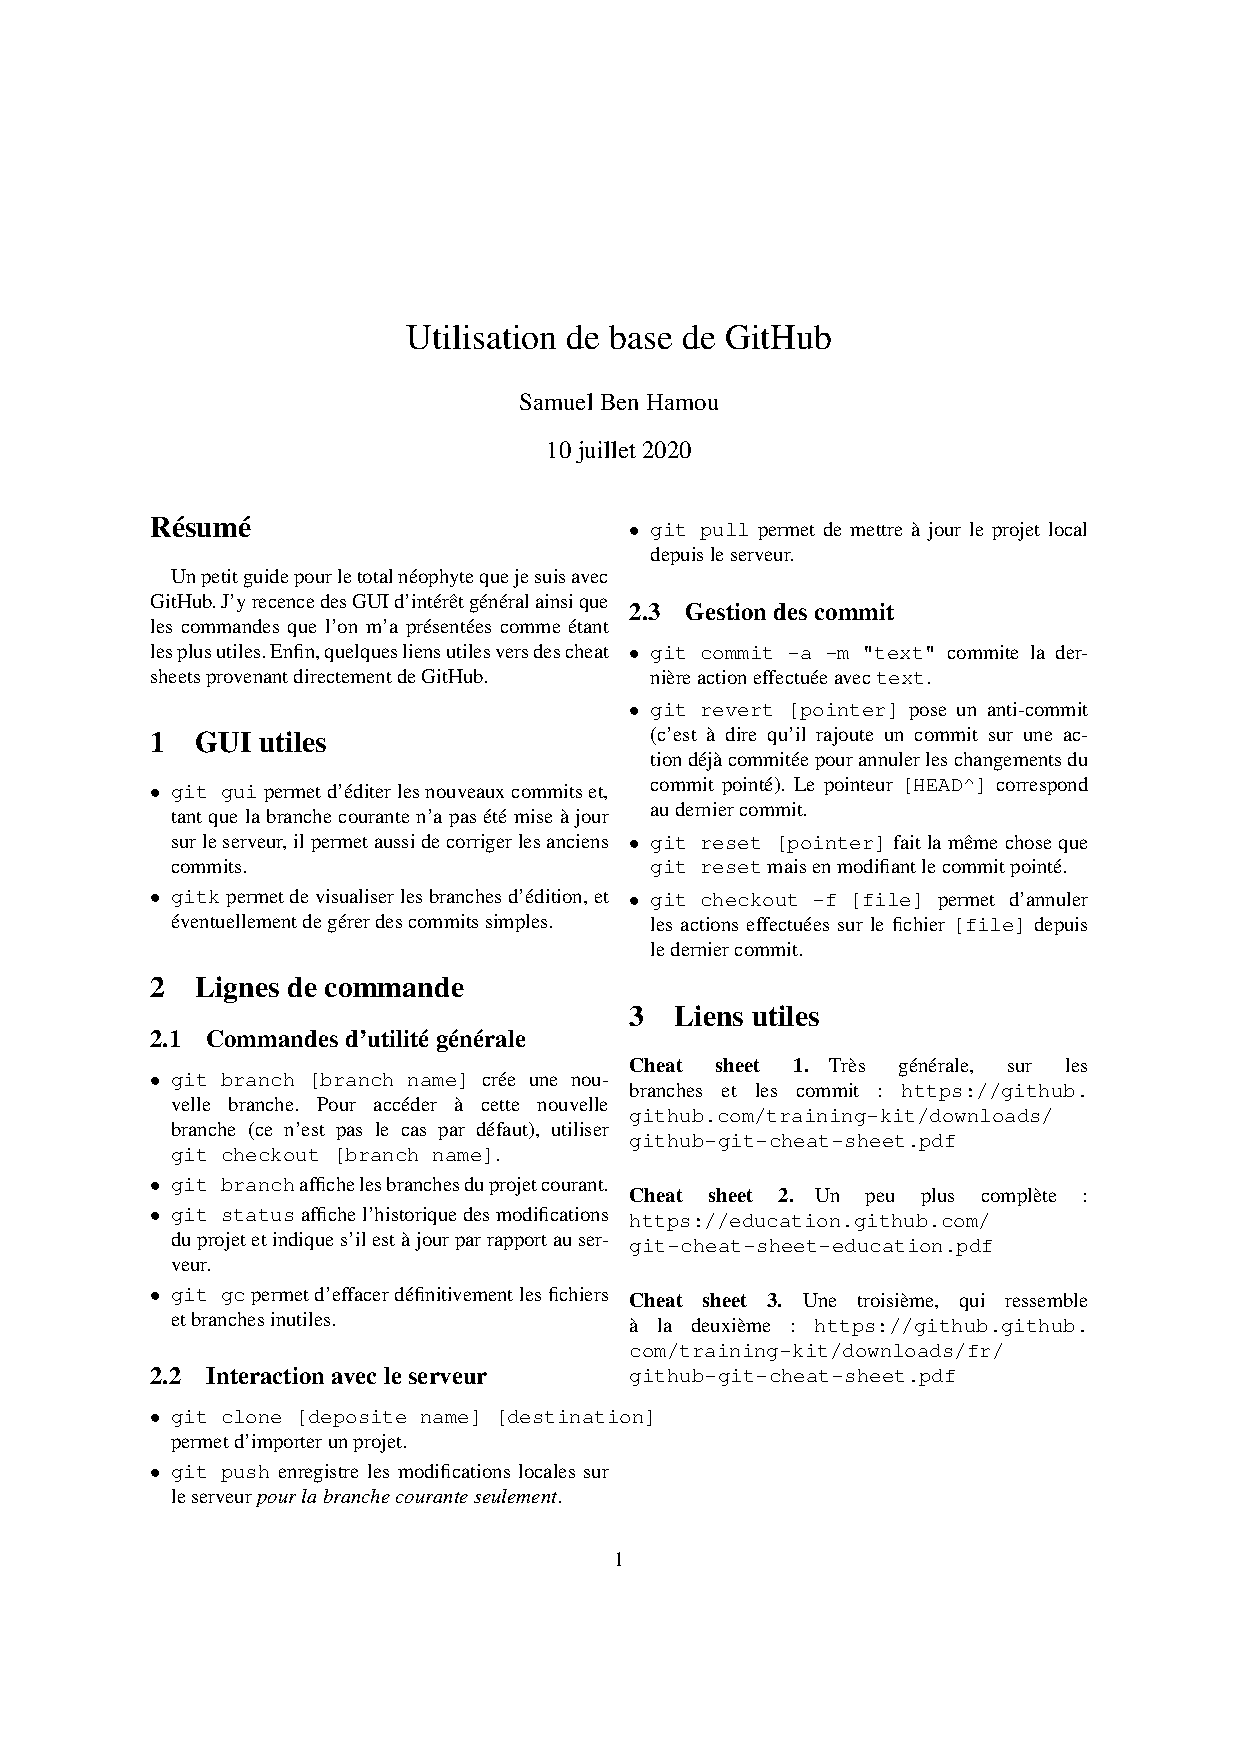
\includepdf[pages=1, nup=1x1, frame=true, scale=0.8, pagecommand=\section{Cheatsheet pour GitLab}\label{gitsheet}]{TutoGitHub.pdf}

\section{Définition de \texttt{Pr}} \label{pr}

\begin{minted}{coq}
Inductive Pr (l:logic) : sequent -> Prop :=
 | R_Ax Γ A : In A Γ -> Pr l (Γ ⊢ A)
 | R_Tr_i Γ : Pr l (Γ ⊢ True)
 | R_Fa_e Γ A : Pr l (Γ ⊢ False) ->
                  Pr l (Γ ⊢ A)
 | R_Not_i Γ A : Pr l (A::Γ ⊢ False) ->
                   Pr l (Γ ⊢ ~A)
 | R_Not_e Γ A : Pr l (Γ ⊢ A) -> Pr l (Γ ⊢ ~A) ->
                   Pr l (Γ ⊢ False)
 | R_And_i Γ A B : Pr l (Γ ⊢ A) -> Pr l (Γ ⊢ B) ->
                   Pr l (Γ ⊢ A/\B)
 | R_And_e1 Γ A B : Pr l (Γ ⊢ A/\B) ->
                    Pr l (Γ ⊢ A)
 | R_And_e2 Γ A B : Pr l (Γ ⊢ A/\B) ->
                    Pr l (Γ ⊢ B)
 | R_Or_i1 Γ A B : Pr l (Γ ⊢ A) ->
                   Pr l (Γ ⊢ A\/B)
 | R_Or_i2 Γ A B : Pr l (Γ ⊢ B) ->
                   Pr l (Γ ⊢ A\/B)
 | R_Or_e Γ A B C :
     Pr l (Γ ⊢ A\/B) -> Pr l (A::Γ ⊢ C) -> Pr l (B::Γ ⊢ C) ->
     Pr l (Γ ⊢ C)
 | R_Imp_i Γ A B : Pr l (A::Γ ⊢ B) ->
                     Pr l (Γ ⊢ A->B)
 | R_Imp_e Γ A B : Pr l (Γ ⊢ A->B) -> Pr l (Γ ⊢ A) ->
                   Pr l (Γ ⊢ B)
 | R_All_i x Γ A : ~Names.In x (fvars (Γ ⊢ A)) ->
                   Pr l (Γ ⊢ bsubst 0 (FVar x) A) ->
                   Pr l (Γ ⊢ ∀A)
 | R_All_e t Γ A : Pr l (Γ ⊢ ∀A) -> Pr l (Γ ⊢ bsubst 0 t A)
 | R_Ex_i t Γ A : Pr l (Γ ⊢ bsubst 0 t A) -> Pr l (Γ ⊢ ∃A)
 | R_Ex_e x Γ A B : ~Names.In x (fvars (A::Γ⊢B)) ->
      Pr l (Γ ⊢ ∃A) -> Pr l ((bsubst 0 (FVar x) A)::Γ ⊢ B) ->
      Pr l (Γ ⊢ B)
 | R_Absu Γ A : l=Classic -> Pr l (Not A :: Γ ⊢ False) ->
                  Pr l (Γ ⊢ A).
\end{minted}

\section{Définition des formules} \label{form}

\begin{minted}{coq}
Inductive term :=
  | FVar : variable -> term (** Free variable (global name) *)
  | BVar : nat -> term (** Bounded variable (de Bruijn indices) *)
  | Fun : function_symbol -> list term -> term.

Inductive formula :=
  | True
  | False
  | Pred : predicate_symbol -> list term -> formula
  | Not : formula -> formula
  | Op : op -> formula -> formula -> formula
  | Quant : quant -> formula -> formula.
  
Definition Iff a b := Op And (Op Impl a b) (Op Impl b a). 

Notation "~ f" := (Not f) : formula_scope.
Infix "/\" := (Op And) : formula_scope.
Infix "\/" := (Op Or) : formula_scope.
Infix "->" := (Op Impl) : formula_scope.
Infix "<->" := Iff : formula_scope.

Notation "# n" := (BVar n) (at level 20, format "# n") : formula_scope.

Notation "∀ A" := (Quant All A)
 (at level 200, right associativity) : formula_scope.
Notation "∃ A" := (Quant Ex A)
 (at level 200, right associativity) : formula_scope.
\end{minted}

\section{Preuve de \texttt{ZeroRight} : avant-après}\label{beforeafter_zeroright}

La preuve originelle était :
\begin{minted}{coq}
Lemma ZeroRight :
  IsTheorem J PeanoTheory
            (∀ (#0 = #0 + Zero)).
Proof.
  unfold IsTheorem.
  split.
  + unfold Wf. split; [ auto | split; auto ].
  + exists ((PeanoAx.induction_schema (#0 = #0 + Zero))::axioms_list).
    split.
    - apply Forall_forall.
      intros. destruct H.
      * simpl. unfold IsAx.
        right. exists (#0 = #0 + Zero).
        split; [ auto | split ; [ auto | auto ] ].
      * simpl. unfold IsAx. left. exact H.
    - apply R_Imp_e with
      (A := (nForall (Nat.pred (level (# 0 = # 0 + Zero)))
       ((∀ bsubst 0 Zero (# 0 = # 0 + Zero)) /\
        (∀ # 0 = # 0 + Zero -> bsubst 0 (Succ (# 0)) (# 0 = # 0 + Zero))))).
      * apply R_Ax. unfold induction_schema. apply in_eq.
      * simpl. apply R_And_i. cbn.
        change (Fun "O" []) with Zero.
        apply R_All_i with (x := "x").
        ++ compute. inversion 1.
        ++ cbn. change (Fun "O" []) with Zero.
           eapply R_Imp_e. set (hyp := (_ -> _)%form).
           assert ( sym : Pr J (hyp::axioms_list ⊢ ∀∀ (#1 = #0 -> #0 = #1))).
           { apply R_Ax. compute; intuition. }
           apply R_All_e with (t := Zero + Zero) in sym. cbn in sym.
           apply R_All_e with (t := Zero) in sym. cbn in sym. exact sym.
           -- reflexivity.
           -- reflexivity.
           -- set (hyp := (_ -> _)%form). change (Fun "O" []) with Zero.
              change (Zero + Zero = Zero) with (bsubst 0 Zero (Zero + #0 = #0)).
              apply R_All_e. reflexivity.
              apply R_Ax. compute; intuition.
       ++ cbn. change (Fun "O" []) with Zero.
          apply R_All_i with (x := "y").
          -- compute. inversion 1.
          -- cbn. change (Fun "O" []) with Zero.
             apply R_Imp_i. set (H1 := FVar _ = _). set (H2 := _ -> _).
             assert (hyp : Pr J
                              (H1 :: H2 :: axioms_list ⊢ Fun "S" [FVar "y"] =
                               Fun "S" [FVar "y" + Zero] /\
                               Fun "S" [FVar "y" + Zero] = Fun "S" [FVar "y"] + Zero)).
             { apply R_And_i.
               - assert (AX4 : Pr J (H1 :: H2 :: axioms_list ⊢ ax4)).
                 { apply R_Ax. compute; intuition. }
                 apply R_Imp_e with (A := (FVar "y" = FVar "y" + Zero)%form);
                   [ | apply R_Ax; compute; intuition ].
                 unfold ax4 in AX4. apply R_All_e with (t := FVar "y") in AX4; [ | auto ].
                 apply R_All_e with (t := FVar "y" + Zero) in AX4; [ | auto ].
                 cbn in AX4. exact AX4. 
               - apply R_Imp_e with (A := Fun "S" [FVar "y"] + Zero = Fun "S" [FVar "y" + Zero]).
                 + assert (AX2 : Pr J (H1 :: H2 :: axioms_list ⊢ ax2)).
                   { apply R_Ax. compute; intuition. }
                   unfold ax2 in AX2.
                   apply R_All_e with (t := Fun "S" [FVar "y"] + Zero) in AX2; [ | auto ].
                   apply R_All_e with (t := Fun "S" [FVar "y" + Zero]) in AX2; [ | auto ].
                   cbn in AX2. exact AX2.
                 + assert (AX10 : Pr J (H1 :: H2 :: axioms_list ⊢ ax10)).
                   { apply R_Ax. compute; intuition. }
                   unfold ax10 in AX10.
                   apply R_All_e with (t:= FVar "y") in AX10; [ | auto ].
                   apply R_All_e with (t := Zero) in AX10; [ | auto ].
                   cbn in AX10. exact AX10. }
             apply R_Imp_e with
             (A :=  Fun "S" [FVar "y"] = Fun "S" [FVar "y" + Zero] /\
                    Fun "S" [FVar "y" + Zero] = Fun "S" [FVar "y"] + Zero).
             ** assert (AX3 : Pr J (H1 :: H2 :: axioms_list ⊢ ax3)).
                { apply R_Ax. compute; intuition. }
                unfold ax3 in AX3.
                apply R_All_e with (t:= Fun "S" [FVar "y"]) in AX3; [ | auto ].
                apply R_All_e with (t := Fun "S" [FVar "y" + Zero]) in AX3; [ | auto ].
                apply R_All_e with (t := Fun "S" [FVar "y"] + Zero) in AX3; [ | auto ].
                cbn in AX3. exact AX3.
             ** exact hyp.
 Qed.    
\end{minted}
et en fin de stage, elle était devenue
\begin{minted}{coq}
Lemma ZeroRight :
  IsTheorem J PeanoTheory
            (∀ (#0 = #0 + Zero)).
Proof.
 thm.
 rec.
 + sym.
   inst_axiom ax9 [Zero].
 + app_R_All_i "y" y.
   apply R_Imp_i. set (H1 := _ = _).
   sym.
   trans (Succ (y + Zero)).
   - inst_axiom ax10 [y; Zero].
   - ahered.
     sym.
     apply R_Ax.
     apply in_eq.
Qed.
\end{minted}

\section{Syntaxe et règles de typage du $\lambda$-calcul utilisé} \label{lambda}

La syntaxe des $\lambda$-termes est la suivante :
\begin{align*}
u, v, \ldots ::&= x, y, \ldots & \text{variables}\\
&| \; uv & \text{application} \\
&| \; \lambda x \cdot u & \text{abstraction} \\
&| \; \nabla u & \text{nabla} \\
&| \; \langle u, v \rangle & \text{couple} \\
&| \; \pi_1 u & \text{première projection} \\
&| \; \pi_2 u & \text{seconde projection} \\
&| \; \mathtt{case} \, u \, \mathtt{of} \, \iota_1 x_1 \mapsto v_1 \; | \; \iota_2 x_2 \mapsto v_2 & \text{filtrage par motif} \\
&| \; \iota_1 u & \text{première injection} \\
&| \; \iota_2 u & \text{seconde injection}
\end{align*} et celle des types est \begin{align*}
\sigma, \tau, \ldots ::&= a, b, \ldots & \text{variables de type} \\
&| \; \sigma \Rightarrow \tau & \text{type flèche} \\
&| \; \bot & \text{faux} \\
&| \; \sigma \wedge \tau & \text{type conjonction} \\
&| \; \sigma \vee \tau & \text{type disjonction}.
\end{align*}

Les règles de typage sont :
\[ \begin{array}{lcr}
\text{\begin{prooftree}
\infer0[var]{\Gamma, x : \tau \vdash x : \tau}
\end{prooftree}} &
\text{\begin{prooftree}
\hypo{\Gamma \vdash u : \sigma \Rightarrow \tau}
\hypo{\Gamma \vdash v : \sigma}
\infer2[app]{\Gamma \vdash uv : \tau}
\end{prooftree}} &
\text{\begin{prooftree}
\hypo{\Gamma, x : \sigma \vdash u : \tau}
\infer1[abs]{\Gamma \vdash \lambda x \cdot u : \sigma \Rightarrow \tau}
\end{prooftree}} \\
& & \\
&
\text{\begin{prooftree}
\hypo{\Gamma \vdash u : \bot}
\infer1[$\nabla$]{\Gamma \vdash \nabla u : \tau}
\end{prooftree}} & \\
& & \\
\text{\begin{prooftree}
\hypo{\Gamma \vdash u : \sigma \wedge \tau}
\infer1[$\pi_1$]{\Gamma \vdash \pi_1 u : \sigma}
\end{prooftree}} &
\text{\begin{prooftree}
\hypo{\Gamma \vdash u : \sigma \wedge \tau}
\infer1[$\pi_2$]{\Gamma \vdash \pi_2 u : \tau}
\end{prooftree}} &
\text{
\begin{prooftree}
\hypo{\Gamma \vdash u : \sigma}
\hypo{\Gamma \vdash v : \tau}
\infer2[paire]{\Gamma \vdash \langle u, v \rangle : \sigma \wedge \tau}
\end{prooftree}}\\
& & \\
\text{
\begin{prooftree}
\hypo{\Gamma \vdash u : \sigma}
\infer1[$\iota_1$]{\Gamma \vdash \iota_1 u : \sigma \vee \tau}
\end{prooftree}} & &
\text{
\begin{prooftree}
\hypo{\Gamma \vdash u : \tau}
\infer1[$\iota_2$]{\Gamma \vdash \iota_2 u : \sigma \vee \tau}
\end{prooftree}} \\
& & \\
&
\text{
\begin{prooftree}
\hypo{\Gamma \vdash u : \sigma \vee \tau}
\hypo{\Gamma, x_1 : \sigma \vdash v_1 : \mu}
\hypo{\Gamma, x_2 : \tau \vdash v_2 : \mu}
\infer3[pattern]{\Gamma \vdash \mathtt{case} \, u \, \mathtt{of} \, \iota_1 x_1 \mapsto v_1 \; | \; \iota_2 x_2 \mapsto v_2 : \mu}
\end{prooftree}} &
\end{array} \]

\end{document}
